
\documentclass[12pt]{article}
\usepackage[utf8]{inputenc}
\usepackage[spanish]{babel}
\usepackage{graphicx}
\usepackage{wrapfig}

\usepackage{ulem} % tachado
\graphicspath{ {images/} }
\usepackage{amssymb, amsmath}
\usepackage{tcolorbox}
\usepackage{multicol}
\usepackage{amsfonts}




\title{CUESTIONARIO DE FÍSICA 1\\
Primero de bachillerato A,B y C}
\author{Ing. Luis Fabian Cacuango Eugenio\footnote{fabiancacuango1@gmail.com \quad whatsApp: 0989952725 \quad Web: www.fismatt.com}}
\date{\today}

\begin{document}
\begin{figure}
    \centering
    
\includegraphics[scale=0.5] {14.jpg}
\end{figure}

\maketitle % codigo para crear encabezado

\section*{Nombre : \rule{100mm}{0.1mm}}
\section*{Curso :\rule{110mm}{0.1mm}} 
\newpage 
\tableofcontents %codigo para crear indice
\listoffigures


\newpage 
\section{MAGNITUDES FÍSICAS Y UNIDADES }
\subsection{MAGNITUD:}

 Es toda propiedad de los cuerpos que se puede medir. Por ejemplo: temperatura, velocidad, masa, peso, etc.
 \subsection{MEDIR:} Es comparar la magnitud con otra similar, llamada unidad, para averiguar cuántas veces la contiene. 
\subsection{UNIDAD:}
 Es una cantidad que se adopta como patrón para comparar con ella cantidades de la misma especie. 
 
 \begin{tcolorbox}[colback=red!15!]
 
 
 \subsection*{Ejemplo: } 
 Cuando decimos que un objeto mide dos metros $2m$
 
\begin{align*}
\intertext{ oberve que los $2m$ es dos veces mayor que la unidad}
2m\\ \intertext{el dos es un numero que pertenece al conjunto de los numeros $\mathbb{R}$}
2\\
\intertext{La m es el simbolo del metro que pertenece a la magnitud de longitud}
m 
\end{align*}
 
 




  
 estamos indicando que es dos veces mayor que la unidad tomada como patrón, en este caso el metro.
 \end{tcolorbox}
 
 
 \begin{tcolorbox}[colback=red!15!white]
 \centering
  \subsection*{ACTIVIDAD 1}
 \end{tcolorbox}


 \begin{enumerate}
\item Uno de los parámetro no corresponde a una magnitud
\begin{multicols}{2}
\begin{enumerate}
\item Longitud
\item Masa 
\item Tiempo
\item Temperatura
\item velocidad
\item Intensidad de corriente

\end{enumerate}
\end{multicols}
\item ¿Cuál es la diferencia entre magnitud y unidad de medida?\\
\rule{110mm}{0.1mm}\\



\item Escriba 3 ejemplos de magnitud. 
Ejemplo: Tiempo t\\
\rule{110mm}{0.1mm}\\



\item Escriba 3 ejemplos de unidad.
Ejemplo: segundo  s\\
\rule{110mm}{0.1mm}\\
\rule{110mm}{0.1mm}\\

\end{enumerate}


 
 
 
 
 \section{MAGNITUDES FUNDAMENTALES}
 En el cuadro siguiente puedes ver las magnitudes fundamentales del SI, la unidad de cada una de ellas y la abreviatura que se emplea para representarla:
 

 
 \begin{table}[h]
\begin{center}
\begin{tabular}{ c| c| c|  c }
Magnitud fundamental& S. dimension  & Unidad SI & S. Unidad \\ \hline
Longitud & L& metro & $m$ \\
Masa  &M& Kilogramo & $kg$ \\
Tiempo &T& Segundos & s \\
Temperatura & & Kelvin &$k$\\
Intensidad de corriente &I& Amperio & $A$\\

\hline
\end{tabular}
\caption{Magnitudes del sistema Internacional(SI)}
\label{tab:Magnitudes del sistema internacional SI}
\end{center}
\end{table}
 
 
 

 \begin{tcolorbox} [colback=red!15!white]
 \centering
 \section*{Actividad 2}
  \end{tcolorbox}
 \begin{enumerate}
     \item Entre las alternativas, una de las unidades no corresponde a las magnitudes fundamentales del sistema internacional:
     \begin{multicols}{2}
     \begin{enumerate}
         \item metro
         \item tiempo
         \item segundo
         \item kilogramo
              \end{enumerate}
     \end{multicols}
     
      
     
 
     \item Entre las alternativas, una de las magnitudes no corresponde a las magnitudes fundamentales del sistema internacional:
     \begin{multicols}{2}
     \begin{enumerate}
         \item metro
         \item tiempo
         \item Masa
         \item Longitud
              \end{enumerate}
     \end{multicols}
      
      
      \item ¿Qué magnitud está mal asociada a su unidad base en el S.I.?\\
      Selecciona una de las siguientes respuestas posibles:
      \begin{multicols}{2}
     \begin{enumerate}
         \item Longitud - metro
         \item Tempo - tempo
         \item Masa - kilogramo
         \item Longitud - centímetro
              \end{enumerate}
     \end{multicols}
      
      \item Entre las unidades mencionadas, señala la que pertenece a una unidad base en el S.I.\\
      Selecciona una de las siguientes respuestas posibles:
       \begin{multicols}{2}
     \begin{enumerate}
         \item Longitud - centímetro
         \item Tempo - horas
         \item Masa - gramo
         \item Longitud - metro
              \end{enumerate}
     \end{multicols}
      
     \item ¿Cuál de las unidades no corresponde a una unidad fundamental en el S.I.?\\
     Selecciona una de las siguientes respuestas posibles:
        \begin{multicols}{2}
     \begin{enumerate}
         \item metro - longitud
         \item hora - h
         \item centímetros - cm
         \item kilogramos - kg
         \item kelvin - k
         \item Amperio - A
         
              \end{enumerate}
     \end{multicols}
      
     \item  Un estudiante determinado medía 20 pulg de largo cuando nació. Ahora tiene 5 pies y 4 pulg y tiene 18 años de edad. ¿Cuántos centímetros creció, en promedio, por año?
     \begin{multicols}{2}
     \begin{enumerate}
     \item $6.2 cm$  
      \item $8.2 cm$
      \item $6.7 cm$
      \item $6.5 cm$
        \end{enumerate}
     \end{multicols}
     
     
       \end{enumerate}
      

 


\subsection{múltiplos y los submúltiplos del metro.} 
\subsubsection{Múltiplos}
Los múltiplos son las unidades de medida más grandes que el metro.
\subsubsection{Submúltiplos}
Los submúltiplos son las unidades de medida más pequeñas que el metro. 
\begin{table}[h]
    \centering
    \begin{tabular}{c|c|c|l}
         Prefijo & símbolo&factor  & equivalencia decimal  \\\hline
        Exa &  E & $10^{18}$& $1000000000000000000$\\
        peta &  P & $10^{15}$& $1000000000000000$\\
        tera &  T & $10^{12}$& $1000000000000$\\
        giga &  G & $10^{9}$& $1000000000$\\
        mega &  M & $10^{6}$& $1000000$\\
        kilo &  K & $10^{3}$& $1000$\\
        hecto &  H & $10^{2}$& $100$\\
        deca & da & $10$& $10$\\
        \textbf{Sin prefijo} &   & $1$& $1$\\
        deci &  d & $10^{-1}$& $0.1$\\
        centi&  c & $10^{-2}$& $0.01$\\
        mili&  m & $10^{-3}$& $0.001$\\
        micro & u & $10^{-6}$& $0.000001$\\
        nano & n  & $10^{-9}$& $0.000000001$ \\
        \hline
    \end{tabular}
    \caption{Tabla de múltiplos y los submúltiplos }
    \label{tab:múltiplos y los submúltiplos}
\end{table}

\begin{tcolorbox}[colback=red!15!]
\textbf{Ejemplo 1} : convierte 10000 metros a kilómetros
 
 
\begin{equation*} \label{vonverción de unidades}
\begin{split}
10000m&\rightarrow km\quad\text{Equivalencia de longitud}\\
10000\xout{m}& = \frac{1km}{10000\xout{m}}\quad\text{simplifica los m y 10000 dividido para 1000} \\
 & =10km        \quad\text{Se obtienen la equivalencia en km}
\end{split}
\end{equation*}
\end{tcolorbox}


  
  
\begin{tcolorbox}[colback=red!15!]
\textbf{ejemplo 2:}
     \begin{equation*}
         \begin{split}
                  &34 m= 34000 mm. \quad\text{Longitud} \\
&9km^2=9000000 m^2 \quad\text{Superficie}   
         \end{split}
     \end{equation*}
     
\textbf{Ejemplo 3:} Realiza la siguiente conversión:$$ 4379  \rightarrow km$$
 \textbf{Primer paso}. determina la equivalencia en este caso seria $1000 m= 1 km$ \\
 \begin{equation*}
  \begin{split}
            &=4379\xout{m}=\dfrac{1km}{1000\xout{m}}\Rightarrow\quad\textbf{simplifica las unidades}\\
        &= \dfrac{4379km}{1000}\Rightarrow\quad\textbf{realiza la division}\\
                &=4.379km \Rightarrow\quad\textbf{finalmente hemos convertido de $m \rightarrow km$}
 \end{split}  
 \end{equation*}
 
 
  \end{tcolorbox}
\begin{tcolorbox}[colback=red!5!white]%,colframe=red!35!black,fonttitle=\bfseries,title= Conteste las siguientes preguntas%]
\centering
\section*{Actividades 3}
\end{tcolorbox}

\begin{enumerate}
    \item Realiza la siguiente conversión: $4379 m \rightarrow km$\footnote{realiza todo el procedimiento en una hoja del cuaderno } 
   
      \begin{enumerate}
      \item$ 4.379km$
      \item $ 43.79 km$ 
      \item  $0.4379 km$
  \end{enumerate}
     
     
    
       
     
     \item Realiza la siguiente conversión: $36 m \rightarrow cm $ 
      \begin{multicols}{2}
  \begin{enumerate}
      \item$ 3600 cm$
      \item $ 360 cm$ 
      \item  $36 000 cm$
  \end{enumerate}
  \end{multicols}
  
  
    
 
  \item Realiza la siguiente conversión $5.9 kg\rightarrow mg $
  \begin{multicols}{2}
  \begin{enumerate}
      \item$ 5 900 000 mg$
      \item $ 590 000 mg$ 
      \item  $590 mg$
  \end{enumerate}
     \end{multicols}
    
    
    
\end{enumerate}




 \subsection{MAGNITUDES DERIVADAS}
 MAGNITUDES DERIVADAS En la siguiente tabla aparecen algunas magnitudes derivadas junto a sus unidades
 \begin{table}[h]
     \centering
     \begin{tabular}{c|c|c}
          \textbf{Magnitud} & \textbf{Unidad} & \textbf{Abreviatura}  \\\hline
          superficie & metro cuadrado & $m^{2}$\\
          
         volumen & metro cubico & $m^{3}$\\
         
           Aceleración&	Metro por segundo cuadrado&	$m/s^{2}$\\
           
            velocidad & metro por segundo & $m/s$\\
            
            Frecuencia&	Hercio&	$Hz$	\\
            
           Fuerza&	Newton&	 	$\dfrac{m\times kg}{s^{2}}$\\
           
          Presión, tensión&	Pascal&	$N/m^{2}$\\
          \hline
  
     \end{tabular}
     \caption{Magnitudes derivadas}
     \label{tab:Magnitudes derivadas}
 \end{table}
 

 
 


  \begin{tcolorbox}[colback=red!5!white]%,colframe=red!35!black,fonttitle=\bfseries,title= Conteste las siguientes preguntas]
  \centering
   \section*{Actividades 4}
   \end{tcolorbox}
    
    
    \begin{enumerate}
        \item Escribe sobre la línea si se trata de longitud o superficie.\\
    
  \centering
  
 $$78 m^2= \rule{40mm}{0.1mm} mm^2:\rule{40mm}{0.1mm}$$
  $$80 km^2= \rule{40mm}{0.1mm} dm^2:\rule{40mm}{0.1mm}$$
  $$ 90 mm= \rule{40mm}{0.1mm} m:\rule{40mm}{0.1mm}$$
   $$  78 dm= \rule{40mm}{0.1mm} m:\rule{40mm}{0.1mm}$$
     $$  98 m^2= \rule{40mm}{0.1mm} mm^2:\rule{40mm}{0.1mm}$$
   $$   78 Gm^2= \rule{40mm}{0.1mm} mm^2:\rule{40mm}{0.1mm}$$
  \end{enumerate}
 
 
\section{MAGNITUD ESCALAR y MAGNITUD VECTORIAL}
Desde otro punto de vista las magnitudes se pueden clasificar en:
\begin{itemize}
    \item{escalares} 
\item vectoriales 
\end{itemize}
\subsection{MAGNITUD ESCALAR}
 Es aquella que se describe completamente con un valor numérico y con una unidad de medida apropiada: 
 \subsection*{Ejemplo:} 
 \begin{itemize}
     \item Tiempo: 5 s, 2 h, 3 min, 7 dias....
     \item Temperatura: 3ºC, 273 K
     \item Masa: 3 g, 4 kg, 10 lb, 2 ton...
 \end{itemize}
 
 \subsection{MAGNITUD VECTORIAL}
 Es aquella que se describe completamente por un valor numérico con la unidad de medida apropiada, más una dirección y sentido. 
 \subsection*{Ejemplo:}
 \begin{itemize}
     \item Fuerza
     \item velocidad \footnote{Las magnitudes vectoriales se representan mediante vectores. }
 \end{itemize}
 

\subsubsection{Elementos de un vector }



\begin{figure}[h]
    \centering
    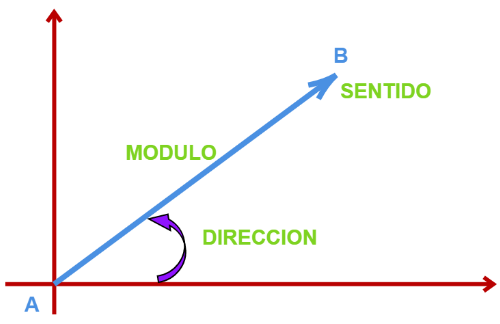
\includegraphics[scale=1.75]{13.png}
    \caption{Elementos de un vector}
    \label{fig:elementos de un vector}
\end{figure}


    \begin{enumerate}

    \item \textbf{Módulo:}  valor numérico de la magnitud vectorial. (La longitud de la flecha) \footnote{los elementos de un vector son valores escalares}
\item \textbf{Dirección:} viene definida por la recta sobre la que está el vector.\footnote{la dirección esta representado por el ángulo} 
\item \textbf{Sentido:} indica hacia donde se dirige el vector. (En una misma dirección hay dos sentidos posibles)\footnote{el sentido esta representado por la flecha} 
\item \textbf{Punto de aplicación:} es el origen del vector.\footnote{Todo vector tiene un origen}
\end{enumerate}




   




 
 
\end{document}
